\documentclass[11pt]{article}


% -- Color scheme

% Color package
\usepackage{xcolor}

% Color scheme definitions

% Default
\definecolor{minimal-main}{HTML}{131313}
\definecolor{minimal-light}{HTML}{F2F2F2}
\definecolor{minimal-contrast}{HTML}{F3F2F5}

% Blue
%\definecolor{minimal-main}{HTML}{1E2839}
%\definecolor{minimal-light}{HTML}{EFF4F9}
%\definecolor{minimal-contrast}{HTML}{F3F2F5}

% Green
%\definecolor{minimal-main}{HTML}{083031}
%\definecolor{minimal-light}{HTML}{DEECE9}
%\definecolor{minimal-contrast}{HTML}{F3F2F5}

% Red
%\definecolor{minimal-main}{HTML}{361222}
%\definecolor{minimal-light}{HTML}{FFE8F2}
%\definecolor{minimal-contrast}{HTML}{F3F2F5}

% Additional color definitions
\definecolor{minimal-black}{HTML}{131313}
\definecolor{minimal-white}{HTML}{F3F2F5}
\definecolor{minimal-red}{HTML}{C43C2D}
\definecolor{minimal-blue}{HTML}{343454}
\definecolor{minimal-yellow}{HTML}{F1C40F}
\definecolor{minimal-green}{HTML}{2D6514}
\definecolor{minimal-beige}{HTML}{D7B6A5}

% Colorbox environments
\usepackage[most]{tcolorbox}


% -- Page layout

% Layout adjustments of page (a4 without margin)
\usepackage[paperheight=842pt, paperwidth=595pt, margin=0pt]{geometry}

% Remove paragraph indentation
\setlength{\parindent}{0pt}

% Interline spacing options
\newcommand{\largespace}{\\[2pt]}
\newcommand{\mediumspace}{\\[-3pt]}
\newcommand{\smallspace}{\\[-5pt]}

% In-box spacing around content
\newcommand{\inboxspacing}{.015\paperheight}

% Horizontal spacing of the boxes (must sum up to 1)
\newcommand{\sideboxwidth}{.35}
\newcommand{\mainboxwidth}{.65}

% Vertical spacing of the boxes (must sum up to 1)
\newcommand{\headboxheight}{.080}
\newcommand{\mainboxheight}{.910}
\newcommand{\footboxheight}{.010}

%   sideboxwidth           mainboxwidth
%  <------------> <---------------------------->
%  _____________________________________________
% |#############################################| ^
% |#############################################| |
% |################## HEADBOX ##################| | headboxheight
% |#############################################| |
% |#############################################| v
% |///////////////                              | ^
% |///////////////                              | |
% |///////////////                              | |
% |///////////////                              | |
% |////   ////////                              | |
% |//// S ////////              M               | |
% |//// I ////////              A               | |
% |//// D ////////              I               | |
% |//// E ////////              N               | | mainboxheight
% |//// B ////////              B               | |
% |//// O ////////              O               | |
% |//// X ////////              X               | |
% |////   ////////                              | |
% |///////////////                              | |
% |///////////////                              | |
% |///////////////                              | |
% |///////////////                              | v
% |#############################################| ^
% |################## FOOTBOX ##################| | footboxheight
% |#############################################| v


% -- Font settings

% Typesetting packages
\usepackage[letterspace=20]{microtype}
\usepackage[T1]{fontenc}

% Raleway font family
\usepackage[semibold]{raleway}
\renewcommand{\familydefault}{\sfdefault}

% Custom font commands
\newcommand{\header}[3]{\uppercase{\textbf{\fontsize{30}{100}{\lsstyle{#1 \hspace{3pt} #2 \hspace{3pt} #3}}}}}
\newcommand{\titlefont}[1]{\uppercase{\textbf{\Large{#1}}}}


% -- Additional packages

% Multirow tables
\usepackage{multirow}

% Settings for entire table columns (e.g \begin{tabular}{>{\footnotesize}rl})
\usepackage{array}

% Tikzpicture graphics
\usepackage{tikz}

% Clickable URLs
\usepackage{hyperref}
\urlstyle{same}


\begin{document}

\begin{tcbposter}[
    poster = {columns=1, rows=1, spacing=0pt},
    boxes = {sharp corners, halign=center, valign=center, boxrule=0pt}
]


% -- Headbox

\posterbox[
    colback=minimal-main,
    halign=center]
    {name=headbox,
    span=1,
    rowspan=\headboxheight}
{

    \color{white}

    \header{Carl}{F.}{Gauss}

    \vspace{-7px}
    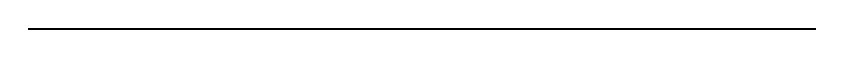
\begin{tikzpicture}
        \draw[fill=white] (-5.0, -0.01) rectangle (5.0, 0.01);
    \end{tikzpicture}
    \vspace{5px}

    \titlefont{The foremost of mathematicians}
}


% -- Sidebox

\posterbox[
    colback=minimal-light,
    valign=top,
    top=\inboxspacing,
    halign=right,
    right=\inboxspacing]
    {name=sidebar,
    below=headbox,
    column=1,
    span=\sideboxwidth,
    rowspan=\mainboxheight}
{

    \begin{tabular}{rl}

        \multicolumn{2}{@{}c@{}}{\scalebox{0.25}{
\begin{tikzpicture}

    \fill[black!10!minimal-white] (-12.3, -16.7) rectangle (12.3, 16.7);
    
    % Blazer
    \fill[minimal-black] (-12.3, -16.7) -- (-12.3, -7.5) -- (-5.5, -4.5) -- (5.5, -4.5) -- (12.3, -7.5) -- (12.3, -16.7) -- cycle;

    % Shirt
    \fill[minimal-white] (-2.5, -16.7) -- (-3.2, -10.5) -- (0.0, -6.5) -- (3.2, -10.5) -- (2.5, -16.7) -- cycle;

    % Neck
    \fill[minimal-beige] (-3.6, -7.5) -- (-3.3, -1.5) -- (3.3, -1.5) -- (3.6, -7.5) -- cycle;

    % Head
    \fill[minimal-beige] (0.0, 5.0) ellipse (6 and 8);

    % Ears
    \fill[minimal-beige, rotate around={10:(-6.25, 4.5)}] (-6.25, 4.5) ellipse (1 and 2.5);
    \fill[minimal-beige, rotate around={-10:(6.25, 4.5)}] (6.25, 4.5) ellipse (1 and 2.5);
    
    % Hair
    \fill[minimal-black] (5.2, 4.0) -- (5.6, 3.9) -- (5.6, 4.5) to[out=70, in=0, looseness=1.4] (0.0, 13.0) to[out=180, in=110, looseness=1.4] (-5.6, 4.5) -- (-5.6, 3.9) -- (-5.2, 4.0) -- (-5.2, 8.5) to[out=340, in=200] (5.2, 8.5) -- cycle;
    
    % Tie
    \fill[minimal-blue] (-2.2, -16.7) -- (-0.6, -8.0) -- (0.6, -8.0) -- (2.2, -16.7) -- cycle;
    \fill[minimal-blue] (0.0, -8.0) circle (1.5);

    % Collar
    \fill[minimal-white] (-5.8, -4.5) -- (-3.5, -3.0) -- (0.0, -6.5) -- (-3.6, -10.5) -- cycle;
    \fill[minimal-white] (5.8, -4.5) -- (3.5, -3.0) -- (0.0, -6.5) -- (3.6, -10.5) -- cycle;

\end{tikzpicture}}} \\
        \mediumspace

        & \titlefont{Contact} \\
        \hline \mediumspace

        \multirow{4}{*}{\scalebox{0.075}{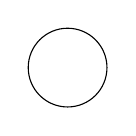
\begin{tikzpicture}
\draw (0,0) circle (0.5);
\end{tikzpicture}}}
            & \textbf{Address} \\
                & Göttingen \\
                & Kingdom of Hanover \\
                & \smallspace

        \multirow{2}{*}{\scalebox{0.075}{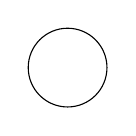
\begin{tikzpicture}
\draw (0,0) circle (0.5);
\end{tikzpicture}}}
            & \textbf{Phone} \\
                & \href{tel:+4901234567891}{+49 012 3456-7891} \\
                & \smallspace

        \multirow{2}{*}{\scalebox{0.075}{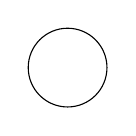
\begin{tikzpicture}
\draw (0,0) circle (0.5);
\end{tikzpicture}}}
            & \textbf{E-Mail} \\
                & \href{mailto:carl.gauss@uni-goe.de}{carl.gauss@uni-goe.de} \\
                & \largespace

        & \titlefont{Personal} \\
        \hline \mediumspace

        \multirow{2}{*}{\scalebox{0.075}{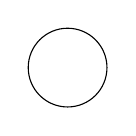
\begin{tikzpicture}
\draw (0,0) circle (0.5);
\end{tikzpicture}}}
            & \textbf{Date of Birth} \\
                & 30/04/1777 \\
                & \smallspace

        \multirow{2}{*}{\scalebox{0.075}{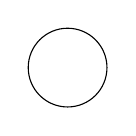
\begin{tikzpicture}
\draw (0,0) circle (0.5);
\end{tikzpicture}}}
            & \textbf{Nationality} \\
                & Holy Roman Empire \\
                & \largespace

        & \titlefont{Platforms} \\
        \hline \mediumspace

        \multirow{2}{*}{\scalebox{0.075}{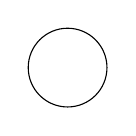
\begin{tikzpicture}
\draw (0,0) circle (0.5);
\end{tikzpicture}}}
            & \textbf{GitHub} \\
                & \href{https://youtu.be/dQw4w9WgXcQ}{CFGauss} \\
                & \smallspace

        \multirow{2}{*}{\scalebox{0.075}{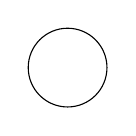
\begin{tikzpicture}
\draw (0,0) circle (0.5);
\end{tikzpicture}}}
            & \textbf{LinkedIn} \\
                & \href{https://youtu.be/dQw4w9WgXcQ}{Carl Friedrich Gauss} \\
                & \largespace

        & \titlefont{Languages} \\
        \hline \mediumspace

        \multirow{2}{*}{\scalebox{0.075}{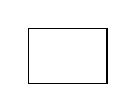
\begin{tikzpicture}
\draw (0,0) rectangle (1,0.7);
\end{tikzpicture}}}
            & \textbf{German} \\
                & Native \\
                & \smallspace

        \multirow{2}{*}{\scalebox{0.075}{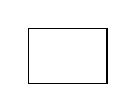
\begin{tikzpicture}
\draw (0,0) rectangle (1,0.7);
\end{tikzpicture}}}
            & \textbf{English} \\
                & Fluent \\
                & \smallspace

        \multirow{2}{*}{\scalebox{0.075}{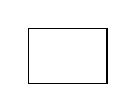
\begin{tikzpicture}
\draw (0,0) rectangle (1,0.7);
\end{tikzpicture}}}
            & \textbf{French} \\
                & Fluent

    \end{tabular}
}


% -- Mainbox

\posterbox[
    colback=white,
    valign=top,
    top=\inboxspacing,
    halign=left,
    left=\inboxspacing]
    {name=mainbox,
    column*=1,
    span=\mainboxwidth,
    below=headbox,
    rowspan=\mainboxheight}
{

    \begin{tabular}{>{\footnotesize}rl}

        & \titlefont{Education} \\
        \hline \mediumspace

        02/1798 - 09/1799
            & \textbf{University of Helmstedt} \\
            & Doctoral dissertation \\
            & Topic: Fundamental theorem of algebra \\
            & Advisor: Johann Friedrich Pfaff \\
            & \smallspace

        04/1795 - 02/1798
            & \textbf{University of Göttingen} \\
            & Study of mathematics \\
            & Construction of regular 17-gon (ruler/compass) \\
            & \smallspace

        04/1788 - 04/1795
            & \textbf{Gymnasium Brunswick}\\
            & Study of high German and Latin \\
            & Stipend from the duke of Brunswick \\
            & \largespace

        & \titlefont{Work Expericence} \\
        \hline \mediumspace

        Since 02/1807
            & \textbf{Astronomical Observatory in Göttingen} \\
            & Full professor of astronomy \\
            & Director of the observatory \\
            & \smallspace

        04/1818 - 08/1826
            & \textbf{State of Hanover} \\
            & Geodesic survey of Hanover \\
            & Triangulation of the entire state \\
            & Invented heliotrope to simplify measurements \\ 
            & \largespace

        & \titlefont{Selected Publications} \\
        \hline \mediumspace
        1832
            & \textbf{The Intensity of the Earth's Magnetic Force} \\
        1827
            & \textbf{General Investigations of Curved Surfaces} \\
        1809
            & \textbf{Theory of the Motion of the Heavenly Bodies} \\
        1801
            & \textbf{Arithmetical Investigations} \\
            & \largespace

        & \titlefont{Awards} \\
        \hline \mediumspace

        1838
            & \textbf{Copley Medal} \\
        1809
            & \textbf{Lalande Prize} \\
            & \largespace

        & \titlefont{Memberships} \\
            \hline \mediumspace
            1853
                & \textbf{American Philosophical Society} \\
                & Elected member \\
            1845
                & \textbf{Royal Institute of the Netherlands} \\
                & Associated member \\
            1822
                & \textbf{American Academy of Arts and Sciences} \\
                & Foreign honorary member \\
            1821
                & \textbf{Royal Swedish Academy of Sciences} \\
                & Foreign member \\
                & \largespace

        & \titlefont{Hobbies} \\
        \hline \mediumspace
            & Astronomical observations and measurements \\
            & Investigation of prime number distribution \\
            & Observation of Earth's magnetic field \\
            & Philology and Russian literature

    \end{tabular}
}


% -- Footbox

\posterbox[colback=minimal-main]
           {name=blankbox2,
           below=sidebar,
           column=1,
           span=1,
           rowspan=\footboxheight}{}

\end{tcbposter}

\end{document}